\documentclass[../mcmpaper]{subfiles}
\begin{document}
	\section{Introduction}
	\subsection{Problem Background}
	The Asian giant hornet is the largest hornet in the world, which is native to East Asia, South Asia, mainland Southeast Asia and some far east parts of the Russian. Recently, it was discovered in the American Northwest at the end of 2019, and there had been lots of sightings in 2020. In fact, the invasion of the Asian giant hornet is not an isolated incident.  In 2004, it first appeared in Europe, and then began to spread to Spain, Belgium, Portugal and Italy, rapidly. According to European studies, the propagation speed of Asian giant hornet can reach 49.5 kilometers per year [2, 11].
	\par
    Even worse, the Asian giant hornet attacks and hunts variety of insects such as bees, bum-blebees, praying mantises and other insects. Moreover, if the Asian giant hornet reach all suitable habitats in North America, the cost for dealing with this disaster in America will ex-ceed \$113.7 millions [1]. Therefore, it is very necessary to find and process the Asian giant hornet effiectively.
    \subsection{Clarifications and Restatements}
    In this problem, we are given the data of observations on the Asian giant hornet, which is perceived by local citizens, including the time, location, latitude and longitude, and the cor- responding observation photos. Washington State Department of Agriculture divided observa- tions into four status based on photos, namely: positive, negative, unverified, and unprocessed. We will solve the following problems based on the historial observations:
    \begin{enumerate}[label=\arabic*., format=\bfseries, itemindent=2\parindent, leftmargin=0pt, topsep=0pt, parsep=0pt]
        \item Based on positive observations and corresponding latitudes and longitudes, combined with the biological characteristics of the Asian giant hornet, forecast the short-term spread of the species and analyze the accuracy of the prediction;
        \item Establish a model for judging whether a photo contains at least an Asian giant hornet, and analyze the image features that make the model output ``Negative'' results;
        \item Based on the above classification model, define the government’s priority in handling citizen observations, for the reason that some unprocessed or unverified observations are most likely to be positive and require the government to explore;
        \item Consider that more sightings have been observed, determine the update method and update frequency of the model;
        \item According to the model above, analyze what indicators of Washington State has achieved, it can be said that the pest has been “eliminated”;
        \item Submit a memorandum to to the Washington State Department of Agriculture to com- prehensively supplement our research results and take corresponding protective measures at the same time.
    \end{enumerate}
    \subsection{Our Work}
    In problem 1, we construct and simulate a time-step diffierence equation with two metrics: \textbf{the resource competition coefficient} and \textbf{the environmental friendliness}. We use this model to predict the distribution of nests in Washington State. Then, we gain the range of activities of a single Asian giant hornet by adding noise. After that, we use the Logistic Growth Model to test the accuracy of the model.
    \par
    We divide problem 2 into two subproblems: \textbf{feature extraction}, \textbf{and image classifi-cation}. In order to reduce the impact of sample imbalance, we apply image flipping and Borderline-SMOTE methods for \textbf{data augmentation} first, and then divide the data into the training set and the validation set (testing set). Next, we \textbf{utilize auto-encoder to collect key features of images}. To prevent over-fitting, we store \textbf{the best performance model} in the testing set for subsequent use. Next, we establish three models, the Binary Logistic Regression, the Support Vector Machine, and the Convolutional Neural Network. After com- paring their accuracy on the testing set, we choose CNN as our image classification model. Finally, we summarize the main features of having negative labels from three aspects: \textbf{species characteristics, subject definition and background softness}.
    \par
    As for problem 3, we take the scope of activities of one-time inspection by the government into account, and conduct Agglomerative Clustering according to the latitude and longitude of each sighting. Then we define the priority of a region based on the positive probabilities of input images.
    \par
    With regard to problem 4, we discuss the effect of updating the model with different time intervals on the testing results, including the loss of auto-encoder and the accuracy of CNN. \textbf{The optimal time interval of updating models is defined as the abscissa corresponding to the extremum of the numerical derivative of the function}, which is the maximum value for auto-encoder, and the opposite for CNN.
    \par
    In terms of problem 5, the number of nests, the range of spatial distribution and the positive ratio in observations can all reflect the growth of pests. We design a number of variables to characterize changes in the number of nests. Since the image recognition model has a certain error probability, we have made a correction based on Bayesian inference.
    \begin{figure}[!ht]
    \centering
    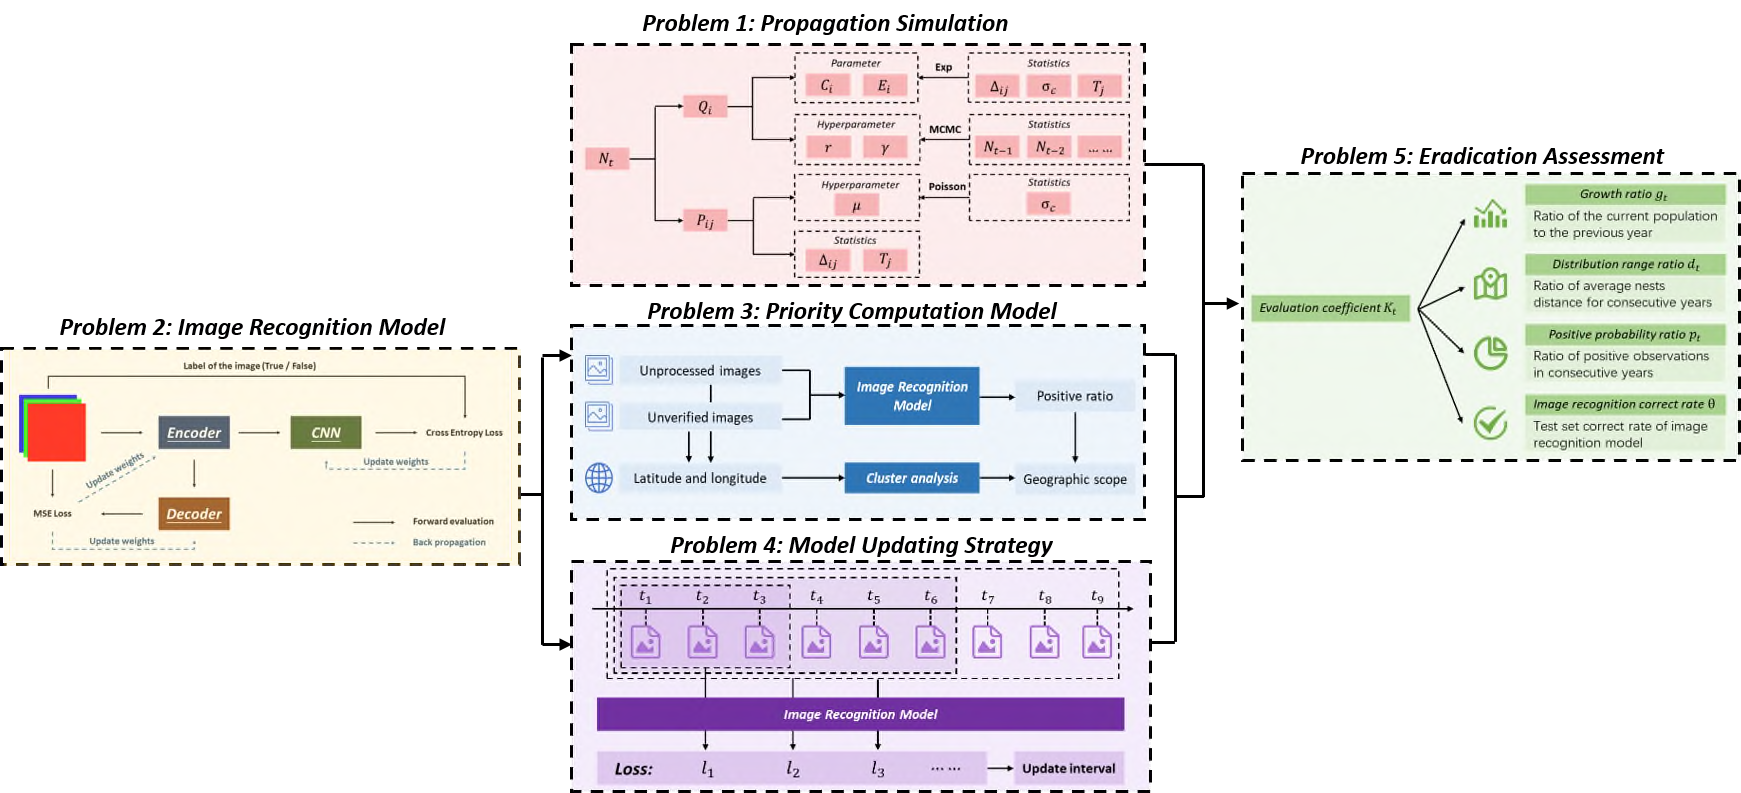
\includegraphics[scale=0.3]{first}
    \caption{The workflow}
    \label{fig:first}
    \end{figure}
	% \begin{Theorem} \label{thm:latex}
	% 	\LaTeX
	% \end{Theorem}
	% \begin{Lemma} \label{thm:tex}
	% 	\TeX .
	% \end{Lemma}
	% \begin{proof}
	% 	The proof of theorem.
	% \end{proof}

\end{document}
%%% Local Variables:
%%% mode: latex
%%% TeX-master: "../mcmpaper"
%%% End:
